\documentclass{article} 
\usepackage{array}
\input{HRCommands}
\newcommand{\BG}{\vbGamma}
\newcommand{\RBar}{\overline{R}}

\graphicspath{{figures/}}

%%%%%%%%%%%%%%%%%%%%%%%%%%%%%%%%%%%%%%%%%%%%%%%%%%%%%%%%%%%%%%%%%%%%%%
% special commands for this document %%%%%%%%%%%%%%%%%%%%%%%%%%%%%%%%% 
%%%%%%%%%%%%%%%%%%%%%%%%%%%%%%%%%%%%%%%%%%%%%%%%%%%%%%%%%%%%%%%%%%%%%%

%**************************************************
%* Document header info ***************************
%**************************************************
\title{Surface Impedance Boundary Conditions in {\sc scuff-em}}
\author {Homer Reid}
\date {May 9, 2012}

%**************************************************
%* Start of actual document ***********************
%**************************************************

\begin{document}
\maketitle

\pagestyle{myheadings}
\markright{Homer Reid: Surface Impedance Boundary Conditions in {\sc scuff-em} }

\begin{abstract}
I consider the implementation of surface-impedance boundary
conditions in the surface-integral-equation formalism
as implemented in {\sc scuff-em}.
I consider formulations for two distinct situations:
\textbf{(a)} ``imperfectly electrically conducting'' (IPEC) bodies,
which are similar to PEC bodies but with some lossiness
introduced,
\textbf{(b)} ``conductive dielectric interfaces'' (CDIs),
which model the effects of thin metal layers lying at the 
interface between two homogeneous material regions.
\end{abstract}

\tableofcontents 

%%%%%%%%%%%%%%%%%%%%%%%%%%%%%%%%%%%%%%%%%%%%%%%%%%%%%%%%%%%%%%%%%%%%%%
%%%%%%%%%%%%%%%%%%%%%%%%%%%%%%%%%%%%%%%%%%%%%%%%%%%%%%%%%%%%%%%%%%%%%%
%%%%%%%%%%%%%%%%%%%%%%%%%%%%%%%%%%%%%%%%%%%%%%%%%%%%%%%%%%%%%%%%%%%%%%
\newpage
\section{IBCs for PEC surfaces}

The usual boundary condition imposed at the surface of a
perfectly electrically conducting (PEC) scatterer is that
the total tangential electric field vanish:
%====================================================================%
\numeq{PECBC1}
 { \vb E_{\parallel}\sups{tot}(\vb x) = 0. }
%====================================================================%

At the surface of an \textit{imperfectly} electrically conducting
(IPEC) scatterer with dimensionless relative surface impedance
$\zeta$, the boundary condition (\ref{PECBC1}) is modified to
read 
%====================================================================%
\numeq{IPECBC1}
{
\vb E_{\parallel}\sups{tot}(\vb x)
= \zeta Z_0 \vbhat{n}\times \vb H\sups{tot}(\vb x)
}
%====================================================================%
where $Z_0\approx 377\,\Omega$ is the impedance of vacuum.

I will refer to (\ref{IPECBC1}) as the ``impedance boundary condition'' (IBC).

%%%%%%%%%%%%%%%%%%%%%%%%%%%%%%%%%%%%%%%%%%%%%%%%%%%%%%%%%%%%%%%%%%%%%%
%%%%%%%%%%%%%%%%%%%%%%%%%%%%%%%%%%%%%%%%%%%%%%%%%%%%%%%%%%%%%%%%%%%%%%
%%%%%%%%%%%%%%%%%%%%%%%%%%%%%%%%%%%%%%%%%%%%%%%%%%%%%%%%%%%%%%%%%%%%%%
\newpage
\section{Two SIE formulations for IPEC bodies}

\subsection{Review: SIE formulation for PEC bodies}

I will consider two distinct SIE formulations for IPEC bodies.
These are both variants of the usual SIE procedure for PEC
bodies, which---by way of review---I summarize thusly:
%
\begin{enumerate}
 \item We introduce an electric surface current $\vb K(\vb x)$ on 
       the surface of a PEC scatterer. This current is related to 
       the total tangential $\vb H$-field according to 
       \numeq{KDef}
       {\vb K(\vb x) = \vbhat{n}\times \vb H\sups{tot}(\vb x).}
 \item We do \textit{not} need to introduce a magnetic surface 
       current; such a current would be proportional to the total
       tangential $\vb E$ field, but this vanishes in view of 
       the boundary condition (\ref{PECBC1}):
       \numeq{NVanishes}
        {\vb N(\vb x) = -\vbhat{n}\times \vb E\sups{tot}(\vb x)\equiv0.}
 \item $\vb K$ gives rise to scattered $\vb E$ and $\vb H$ fields according to
       \begin{align}
        \vb E\sups{scat} &= \int \BG_{\parallel}\supt{EE}(\vb x, \vb x^\prime) 
                            \cdot \vb K(\vb x^\prime) d\vb x^\prime
        \\
        \vb H\sups{scat} &= \int \BG_{\parallel}\supt{ME}(\vb x, \vb x^\prime) 
                            \cdot \vb K(\vb x^\prime) d\vb x^\prime.
       \end{align}
 \item We solve for $\vb K$ by demanding that the scattered field
       to which it gives rise satisfy the boundary condition
       (\ref{PECBC1}):
       \begin{align}
                \vb E_{\parallel}\sups{scat}(\vb x)
            &= -\vb E_{\parallel}\sups{inc}(\vb x)
        \label{PECBC2}
        \intertext{or} 
             \underbrace{
                \int \BG_{\parallel}\supt{EE}(\vb x, \vb x^\prime) 
                     \cdot \vb K(\vb x^\prime) d\vb x^\prime 
                        }_{\BG_{\parallel}\supt{EE} \star \vb K}
            &= - \vb E\sups{inc}(\vb x).
        \label{PECBC3}
        \end{align}
\end{enumerate}

%=================================================
%=================================================
%=================================================
\subsection{First SIE formulation for IPEC bodies}

My first SIE formulation for IPEC bodies 
%
\begin{enumerate}
 \item As in the PEC case, to each IPEC I continue to assign an electric
       surface current $\vb K$ related to the total $\vb H$ field
       by equation (\ref{KDef}).
 \item As in the PEC case, I continue to assign \textit{no} magnetic 
       surface current $\vb N$ to IPEC surfaces.
 \item To determine $\vb K$ from $\vb E\sups{inc}$, I use 
        (\ref{IPECBC1}) in place of (\ref{PECBC1}) and (\ref{PECBC2}).
        This has the effect of replacing (\ref{PECBC3}) with
       %====================================================================%
       \numeq{IPECEquation1}
        {
                 \vbGamma\supt{EE} \star \vb K
      -\zeta Z_0\vbhat{n}\times \vbGamma\supt{ME} \star \vb K
                 = -\vb E\sups{inc} + \zeta Z_0 \vbhat{n}\times \vb H\sups{inc}
        }
       %====================================================================%
\end{enumerate}

%=================================================
%=================================================
%=================================================
\subsection{Second SIE formulation for IPEC bodies}

My alternative SIE formulation for IPEC bodies goes like this:
%
\begin{enumerate}
 \item As before, to each IPEC surface I continue to assign an electric
       surface current $\vb K$ related to the total $\vb H$ field 
       by equation (\ref{KDef}).
 \item Unlike before, I now assign to each IPEC
       surface a nonvanishing magnetic current, which is
       not an independent unknown but is instead
       determined by $\vb K$ via the (\ref{IPECBC1}):
       %====================================================================%
       $$\vb N(\vb x) = -\vbhat{n}\times \vb E\sups{tot}(\vb x)
                      = -\zeta Z_0 \vbhat{n}\times \vb K(\vb x).
       $$
       %====================================================================%
 \item $\vb K$ and $\vb N\equiv \vb N[\vb K]$ give rise to scattered $\vb E$ and 
       $\vb H$ fields according to
       \numeq{EHScat1}
       { \vb E\sups{scat} =
           \BG\supt{EE} \star \vb K
          +\BG\supt{EM} \star \vb N,
          \qquad
         \vb H\sups{scat} =
          \BG\supt{ME} \star \vb K
         +\BG\supt{MM} \star \vb N
       }
%       which I could write alternatively as 
%       \begin{align*}
%         \vb E\sups{scat} &= 
%           \int \left\{ \BG_{\parallel}\supt{EE}(\vb x, \vb x^\prime) 
%                        +Z_s \Big[\vbhat{n}\times \BG_{\parallel}\supt{ME}(\vb x, \vb x^\prime)\Big]
%                \right\}
%                        \cdot \vb K(\vb x^\prime) \,d\vb x^\prime
%         \\
%         \vb H\sups{scat} &= 
%           \int \left\{ \BG_{\parallel}\supt{ME}(\vb x, \vb x^\prime) 
%                        +Z_s \Big[\vbhat{n}\times \BG_{\parallel}\supt{MM}(\vb x, \vb x^\prime)\Big]
%                \right\}
%                        \cdot \vb K(\vb x^\prime) \,d\vb x^\prime
%       \end{align*}
 \item I solve for $\vb K$ by demanding that the scattered fields
       (\ref{EHScat1})
       satisfy the boundary condition (\ref{IPECBC1}):
       $$
           \vb E_{\parallel}\sups{scat}(\vb x) 
            -\zeta Z_0 \vbhat{n}\times \vb H_{\parallel}\sups{scat}(\vb x)
       = 
          -\vb E_{\parallel}\sups{inc}(\vb x) 
            +\zeta Z_0 \vbhat{n}\times \vb H_{\parallel}\sups{inc}(\vb x).
       $$
       or
       \begin{align*}
       \int\bigg\{ &\BG_{\parallel}\supt{EE}(\vb x, \vb x^\prime) 
                   \cdot \vb K(\vb x^\prime)
                   \\
                   &-\zeta Z_0\BG_{\parallel}\supt{ME}(\vb x, \vb x^\prime)
                   \cdot \Big[\vbhat{n}\times \vb K(\vb x^\prime)\Big] 
                   \\
                   &-\zeta Z_0\vbhat{n}\times \BG_{\parallel}\supt{EM}(\vb x, \vb x^\prime) 
                   \cdot \vb K(\vb x^\prime)
                   \\
                   &+\zeta^2 Z_0^2
                   \vbhat{n}\times\BG_{\parallel}\supt{MM}(\vb x, \vb x^\prime)
                   \cdot \Big[\vbhat{n}\times \vb K(\vb x^\prime)\Big]
       \bigg\}
       = -\vb E_{\parallel}\sups{inc}(\vb x) 
            +\zeta Z_0 \vbhat{n}\times \vb H_{\parallel}\sups{inc}(\vb x).
       \end{align*}
\end{enumerate}

%####################################################################%
%####################################################################%
%####################################################################%
\newpage
\section{Example 1: Dielectric film with thin conductive coating layer}

\subsection{Exact solution}
\label{FilmExactSolution}

%####################################################################%
%####################################################################%
%####################################################################%
\begin{figure}[h]
\resizebox{\textwidth}{!}{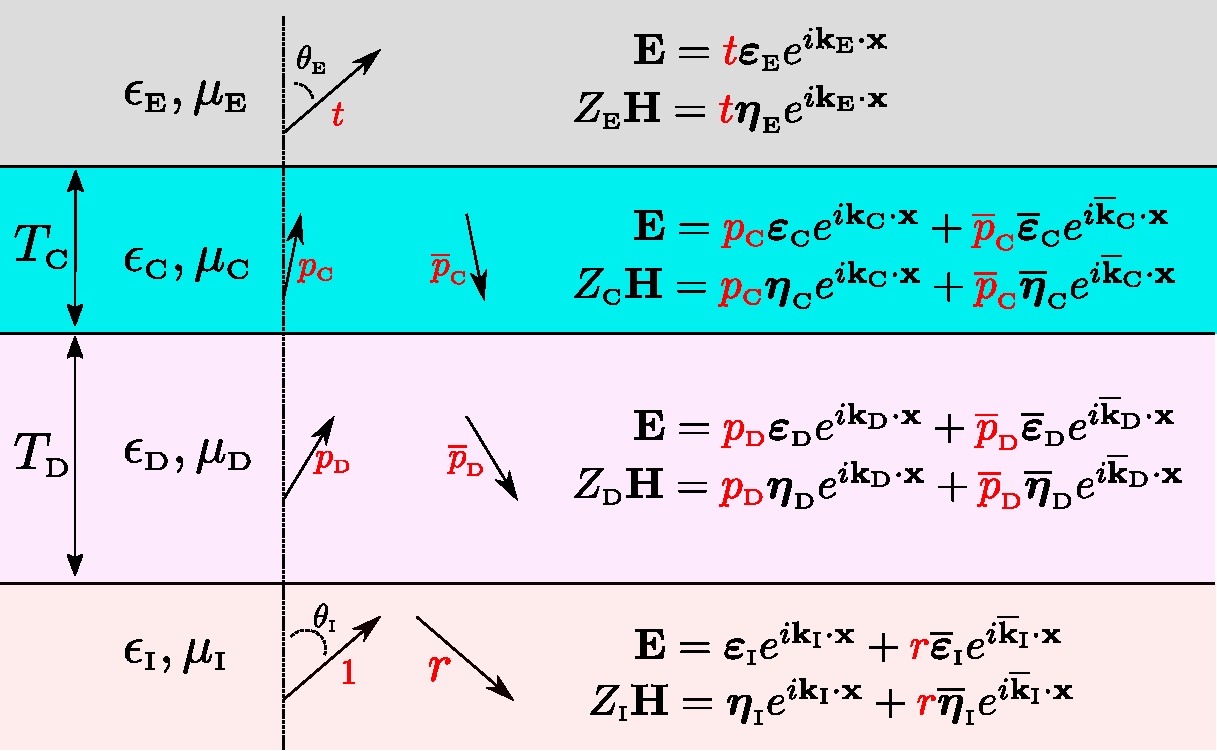
\includegraphics{TwoFilmTransmission.pdf}}
\caption{Transmission through a two-layer film. Eventually I will take
layer C to be thin and highly conductive and will try to model it 
by an infinitesimally thin surface-impedance layer. 
Subscripts: I=initial/incident/interior, D=dielectric, C=conducting, E=exit/exterior.
}
\label{TwoFilmFigure}
\end{figure}
%####################################################################%
%####################################################################%
%####################################################################%

Figure 1 shows a transmission problem in which a plane wave 
emanating from infinite dielectric medium I (for ``initial''
or ``incident'') impinges on a
two-layer film (consisting of a dielectric layer D 
and a conductive layer C with thicknesses 
$T\subt{D,C}$ and relative material properties 
$\{\epsilon,\mu\}\subt{D,C}$)
and is transmitted into region E (for ``exit'' or ``exterior'').
The input parameters are the frequency $\omega$, incidence
angle $\theta\subt{A}$, and incident $\vb E$-field
polarization $\vbVarEps\subt{A}$. I define coordinates
so that the incident wavevector lives in the $xz$ plane.
The propagation and 
polarization vectors in each region ($R=\{I,D,C,E\}$)
are then determined by
%====================================================================%
$$\begin{array}{>{\displaystyle}lc>{\displaystyle}lc>{\displaystyle}lc>{\displaystyle}l}
\vb k\subt{R}
&=& n\subt{R} k_0 \Big(\sin \theta\subt{R} \vbhat{x} + \cos\theta\subt{R} \vbhat{z}\Big)
&\qquad&
\overline{\vb k}\subt{R}
&=& n\subt{R} k_0 \Big(\sin \theta\subt{R} \vbhat{x} - \cos\theta\subt{R} \vbhat{z}\Big)
\\[5pt]
%--------------------------------------------------------------------%
 \vbVarEps\subt{R}\supt{TE}
&=&\vbhat{y}
&\qquad&
 \overline{\vbVarEps}\subt{R}\supt{TE}
&=&\vbhat{y}
\\[5pt]
%--------------------------------------------------------------------%
 \vbVarEps\subt{R}\supt{TM}
&=&\cos\theta\subt{R}\vbhat{x}-\sin\theta\subt{R}\vbhat{z}
&\qquad&
 \overline{\vbVarEps}\subt{R}\supt{TM}
&=&-\cos\theta\subt{R}\vbhat{x}+\sin\theta\subt{R}\vbhat{z}
\\[5pt]
%--------------------------------------------------------------------%
 \vbEta\subt{R}
&=&\vbhat{k}\subt{R} \times \vbVarEps\subt{R}
&\qquad&
 \overline{\vbEta}\subt{R}
&=&\wh{\overline{\vb k}}\subt{R} \times \overline{\vbVarEps}\subt{R}
\end{array}
$$
%====================================================================%
$$\theta\subt{R}=\sin^{-1}\left[\frac{n\subt{I}}{n\subt{R}}\sin\theta\subt{I}\right]$$
%====================================================================%
with
%====================================================================%
$$ k_0=\frac{\omega}{c},
   \qquad n\subt{R}=\sqrt{\epsilon\subt{R} \mu\subt{R}},
   \qquad Z\subt{R}=Z_0\sqrt\frac{\mu\subt{R}}{\epsilon\subt{R}}.
$$
%====================================================================%
For pure-TE or pure-TM polarization, each of the
$\vb E$ and $\vb H$ fields has precisely one nonzero tangential
component.

Matching tangential $\vb E$ and $\vb H$ fields at each of the three
interfaces then yields a linear system of 6 equations 
in the six unknown field-expansion coefficients.
For example, the two equations contributed by the lowermost 
interface read
%====================================================================%
$$\begin{array}{>{\displaystyle}l>{\displaystyle}l>{\displaystyle}l>{\displaystyle}c>{\displaystyle}l}
  -r\overline{\vbVarEps}\subt{I$\parallel$}
 &+p\subt{D}\vbVarEps\subt{D$\parallel$}
 &+\overline{p}\subt{D}\overline{\vbVarEps}\subt{D$\parallel$}
 &=
 & \vbVarEps\subt{I$\parallel$} 
\\[5pt]
  -\frac{r}{Z\subt{I}}\overline{\vbEta}\subt{I$\parallel$}
 &+\frac{p}{Z\subt{D}}\vbEta\subt{D$\parallel$}
 &+\frac{\overline{p}\subt{D}}{Z\subt{D}}\overline{\vbEta}\subt{D$\parallel$}
 &=
 & \frac{1}{Z\subt{I}}\vbEta\subt{I$\parallel$} 
\end{array}$$
%====================================================================%
Assembling the equations for all interfaces gives a 6$\times$6
linear system of the form
%====================================================================%
\numeq{TwoFilmSystem}
{
\left(\begin{array}{p{0.1in}cp{0.1in}}
 &
 \vphantom{ \left(\begin{array}{c} 
                           r \\ p\subt{D} \\ \overline{p}\subt{D} \\
                           p\subt{C} \\ \overline{p}\subt{C} \\ t
                  \end{array}\right)}
  \vb M 
 &
\end{array}\right)
%--------------------------------------------------------------------%
\left(\begin{array}{c}r \\ p\subt{D} \\ \overline{p}\subt{D} \\
                           p\subt{C} \\ \overline{p}\subt{C} \\ t
\end{array}\right)
=
%--------------------------------------------------------------------%
\left(\begin{array}{c}
  \vbVarEps\subt{I$\parallel$}          \\
  \frac{1}{Z_I}\vbEta\subt{I$\parallel$} \\ 
  0 \\ 0 \\ 0 \\ 0 
\end{array}\right)
}
%====================================================================%
that we solve for the field-expansion coefficients.

%====================================================================%
%====================================================================%
%====================================================================%
\subsection*{Results: Transmission through dielectric layer with thin gold film}

Figure \ref{ThinFilmTransmissionData} shows the tangential $\vb E$ and $\vb H$
fields for the geometry of Figure \ref{TwoFilmFigure} with parameters
%====================================================================%
$$ \epsilon\subt{I}=\epsilon\subt{E}=1, \qquad
   \epsilon\subt{D}=10, \qquad
   \epsilon\subt{C}=\epsilon\subs{gold}, \qquad
   T\subt{D}=1 \, \mu\text{m} \qquad
   T\subt{C}=10\text{ nm},
$$
%====================================================================%
i.e. a 1-$\mu$m-thick dielectric layer coated by a thin (10 nm)
layer of gold, with vacuum above and below. The point of these
figures is that the tangential electric field is continuous
across the gold layer, while the magnetic field appears
to suffer a discontinuous jump upon traversing the gold layer.

%####################################################################%
\begin{figure}[H]
\begin{center}
\begin{tabular}{cc}
\resizebox{0.5\textwidth}{!}{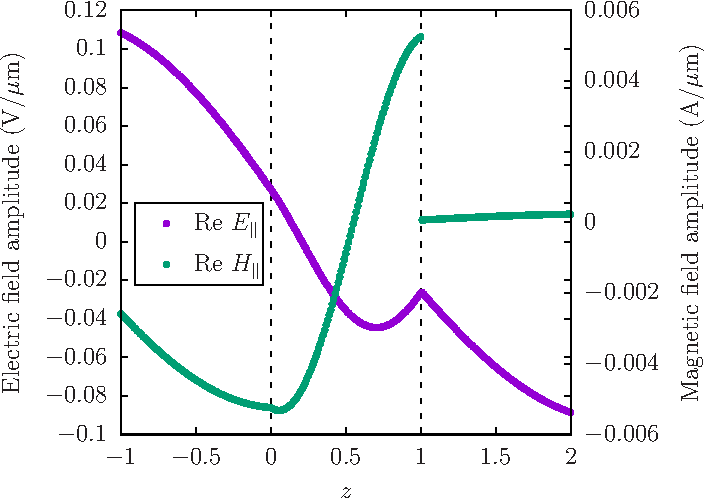
\includegraphics{ThinFilmTransmissionTE.pdf}}
&
\resizebox{0.5\textwidth}{!}{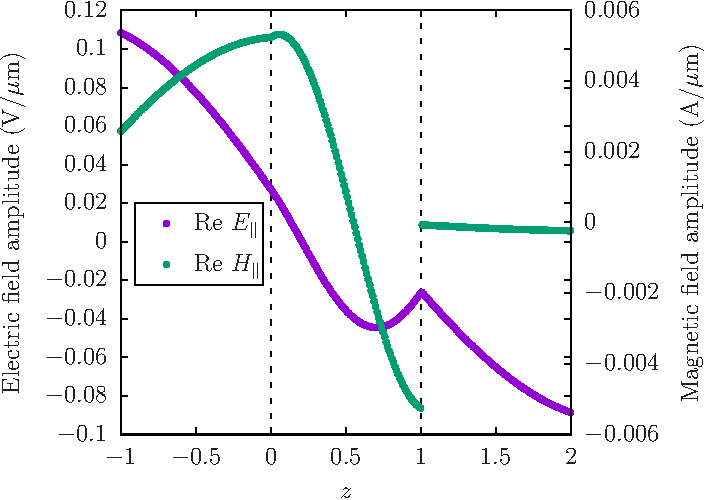
\includegraphics{ThinFilmTransmissionTM.pdf}}
\\
 \textbf{(a)} 
&\textbf{(b)} 
\end{tabular}
\begin{tabular}{c}
\resizebox{0.5\textwidth}{!}{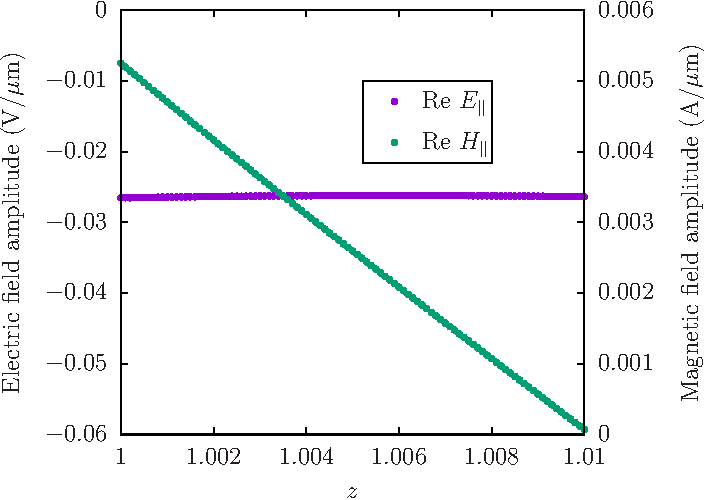
\includegraphics{ThinFilmIBCLayerZoom.pdf}}
 \textbf{(c)} 
\end{tabular}
\caption{Tangential electric (purple) and magnetic (green) fields
         for the geometry of Figure (\ref{TwoFilmFigure})
         irradiated by TE \textbf{(a)} and TM \textbf{(b)} 
         plane waves at incident angle $\theta=\frac{\pi}{4}.$
         The region between the dashed lines is the dielectric
         layer $(\epsilon\subt{D}=10)$. The gold layer lives
         at the right dashed line. In both cases the tangential
         $\vb E$-field is continuous across the gold layer,
         while the tangential $\vb H$-field appears 
         to suffer a discontinuous jump across the layer.
         Zooming in to just the gold layer [plot \textbf{(c)}]
         we see that the $\vb E$-field is nearly constant in 
         the layer, while the $\vb H$-field varies rapidly, giving
         the impression of the discontinuous jumps in
         Figures \textbf{(a,b)}.
         }
\label{ThinFilmTransmissionData}
\end{center}
\end{figure}
%####################################################################%
%####################################################################%
\begin{figure}[H]
\begin{center}
\resizebox{\textwidth}{!}{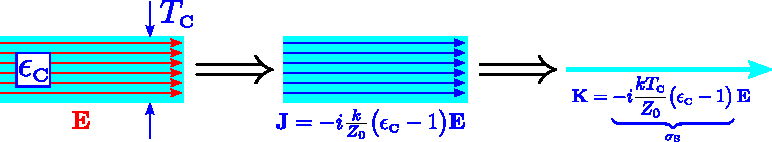
\includegraphics{IBCLayerCurrents.pdf}}
\caption{A constant tangential $\vb E$-field in a thin layer of thickness
         $T\subt{C}$ and relative permittivity $\epsilon$
         produces a constant volume-current density 
         $\vb J=-\frac{ik}{Z_0}(\epsilon-1)\vb E$,
         which we model as an infinitesimally thin sheet
         with surface-current density $\vb K=T\subt{C}\vb J$.}
\label{SurfaceCurrentSchematic}
\end{center}
\end{figure}
%####################################################################%
The fact that the $\vb E$-field is constant throughout the gold
layer [Figure \ref{ThinFilmTransmissionData}\textbf{(c)}] 
suggests the scenario cartooned in Figure \ref{SurfaceCurrentSchematic}:
A constant tangential $\vb E$-field in a thin layer of thickness
$T\subt{C}$ and relative permittivity $\epsilon$
produces a constant volume-current density 
$\vb J=-\frac{ik}{Z_0}(\epsilon-1)\vb E$,
which we model as an infinitesimally thin sheet
with surface-current density $\vb K=T\subt{C}\vb J$.
The effective surface conductivity of the layer
is related to its thickness and bulk conductivity by
%====================================================================%
\numeq{SigmaS}
{\sigma\subt{S}=\frac{|\vb K|}{|\vb E_\parallel|}=
   -\frac{ikT\supt{C}}{Z_0}(\epsilon-1).
}
%====================================================================%

%####################################################################%
%####################################################################%
%####################################################################%
\subsection{IBC solution}
\label{FilmIBCSolution}

%####################################################################%
%####################################################################%
%####################################################################%
\begin{figure}[h]
\resizebox{\textwidth}{!}{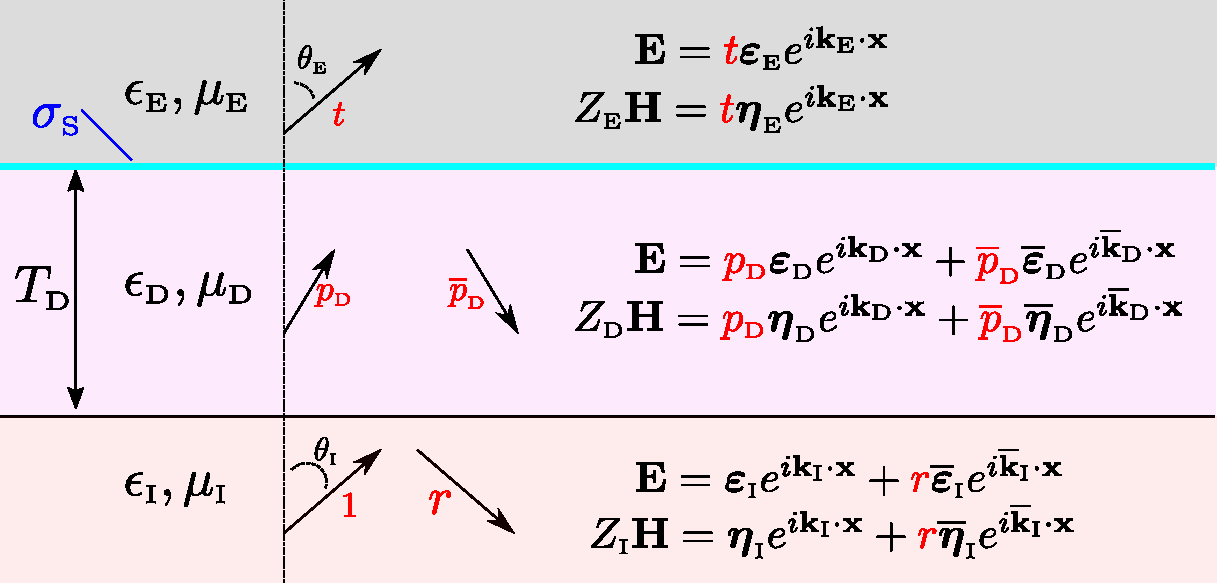
\includegraphics{IBCFilmTransmission.pdf}}
\caption{The two-layer film of the previous section with the 
upper layer modeled as an IBC layer.}
\label{IBCFilmFigure}
\end{figure}
%####################################################################%
%####################################################################%
%####################################################################%
I now consider modeling layer $C$ in Figure \ref{TwoFilmFigure}
as an infinitesimally thin sheet with surface impedance
$\sigma\subt{S}\equiv \frac{1}{Z_0 Z\subt{S}}$
(with $Z\subt{S}$ the dimensionless relative surface impedance),
as shown in Figure \ref{IBCFilmFigure}.
The impedance boundary conditions relate the discontinuity
in the tangential $\vb H$ field across the sheet to the
average $\vb E$-field above and below the sheet:
%####################################################################%
\begin{align}
\vb E\left(z=T\subt{D}^+\right) - \vb E\left(z=T\subt{D}^-\right)
 &=0
\\
\vb H\left(z=T\subt{D}^+\right) - \vb H\left(z=T\subt{D}^-\right)
 &=-\frac{\sigma\subt{S}}{2}\vbhat{z}\times\Big[
  \vb E\left(z=T\subt{D}^+\right) + \vb E\left(z=T\subt{D}^-\right)\Big],
\end{align}
%####################################################################%
or 
%====================================================================%
$$\begin{array}{>{\displaystyle}l>{\displaystyle}l>{\displaystyle}l>{\displaystyle}c>{\displaystyle}l}
  -p\subt{D}\vbVarEps\subt{D$\parallel$}
  \zeta\subt{D}
 &-\overline{p}\subt{D}\overline{\vbVarEps}\subt{D$\parallel$}
  \overline{\zeta}\subt{D}
 &+t\vbVarEps\subt{E$\parallel$} \zeta\subt{E}
 &=
 & 0
\\[5pt]
  -\frac{p\subt{D}}{Z\subt{D}}\vbEta\subt{D$\parallel$}
     \zeta\subt{D}
 &-\frac{\overline{p}\subt{D}}{Z\subt{D}}
     \overline{\vbEta}\subt{D$\parallel$}
     \overline{\zeta}\subt{D}
 &+\frac{t}{Z\subt{E}}\vbEta\subt{E$\parallel$}
     \zeta\subt{E}
 &=
 & -\sigma\subt{S} t \big(\vbhat{z}\times \vbVarEps\subt{e}\big)\zeta\subt{E}
\end{array}
$$
%====================================================================%
$$ \zeta\subt{R}= e^{i\vb k\subt{R}\cdot T\subt{D}\vbhat{z}}, 
   \qquad
   \overline{\zeta}\subt{R}= e^{i\overline{\vb k}\subt{R}\cdot T\subt{D}\vbhat{z}}
$$
%====================================================================%
These two equations replace the last 4 lines of the system 
(\ref{TwoFilmSystem}).

\subsection*{Results: Transmission coefficient in the full calculation and in the IBC approximation}

For the parameters considered above (gold film of thickness $T\subt{C}$ 
on $\epsilon\subt{D}=10$ dielectric layer of thickness 1 $\mu$m),
Figure \ref{IBCVsFullTR} plots the transmission coefficient 
magnitude $|t|$ as computed using the full calculation 
of Section \ref{FilmExactSolution} (filled circles)
and the IBC approximation of 
Section \ref{FilmIBCSolution} (hollow circles)
vs. film thickness $T\subt{C}$.

%####################################################################%
\begin{figure}[H]
\begin{center}
\begin{tabular}{c}
\resizebox{0.5\textwidth}{!}{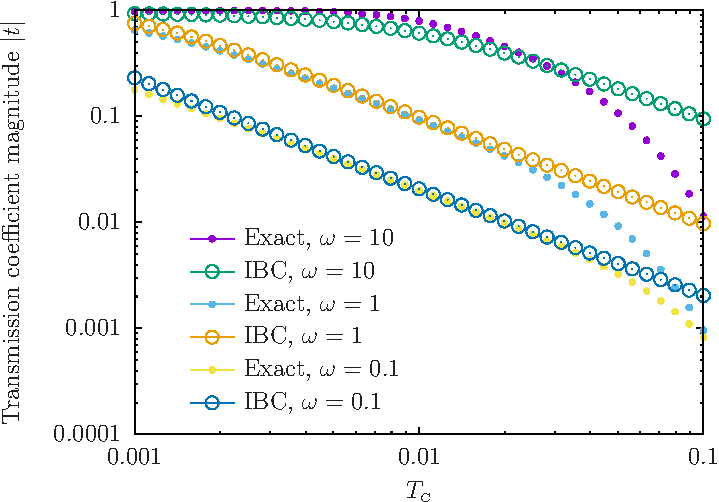
\includegraphics{ExactVsIBC_Theta0_TR.pdf}}\\
\textbf{(a)} $\theta=0$
\end{tabular}

\begin{tabular}{cc}
\resizebox{0.5\textwidth}{!}{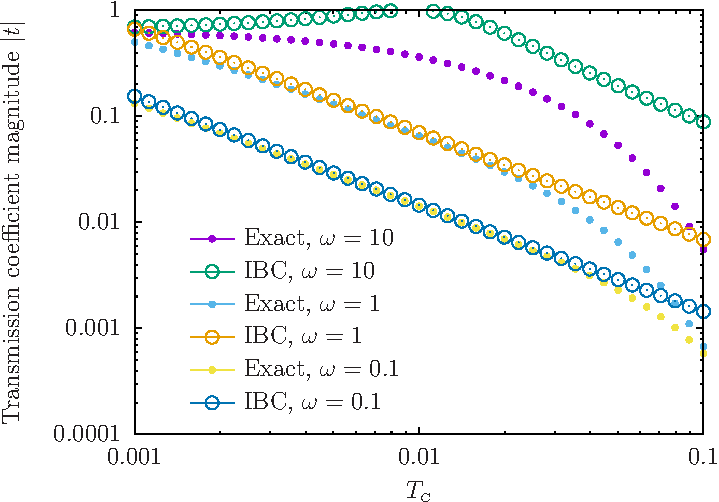
\includegraphics{ExactVsIBC_Theta45TE_TR.pdf}}
&
\resizebox{0.5\textwidth}{!}{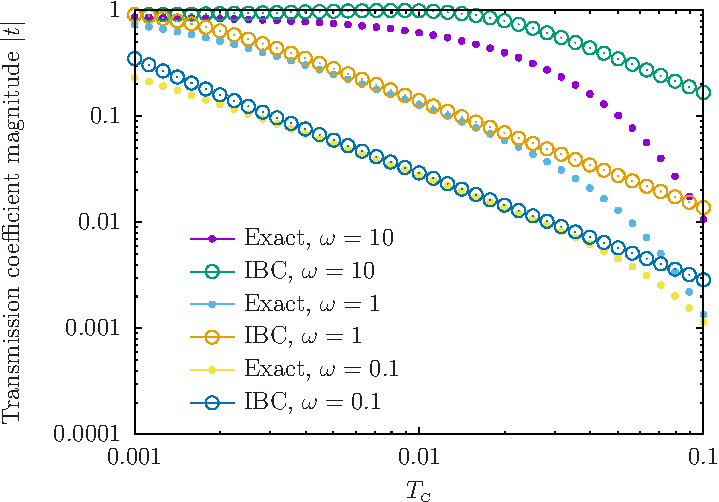
\includegraphics{ExactVsIBC_Theta45TM_TR.pdf}}
\\
\textbf{(b)} $\theta=\frac{\pi}{4}$, TE
&
\textbf{(c)} $\theta=\frac{\pi}{4}$, TE
\end{tabular}
\label{IBCVsFullTR}
\end{center}
\end{figure}
%####################################################################%

%%%%%%%%%%%%%%%%%%%%%%%%%%%%%%%%%%%%%%%%%%%%%%%%%%%%%%%%%%%%%%%%%%%%%%
%%%%%%%%%%%%%%%%%%%%%%%%%%%%%%%%%%%%%%%%%%%%%%%%%%%%%%%%%%%%%%%%%%%%%%
%%%%%%%%%%%%%%%%%%%%%%%%%%%%%%%%%%%%%%%%%%%%%%%%%%%%%%%%%%%%%%%%%%%%%%
\newpage
\section{Example 2: Dielectric sphere with thin conductive coating layer}

%####################################################################%
%####################################################################%
%####################################################################%
\begin{figure}[H]
\resizebox{\textwidth}{!}{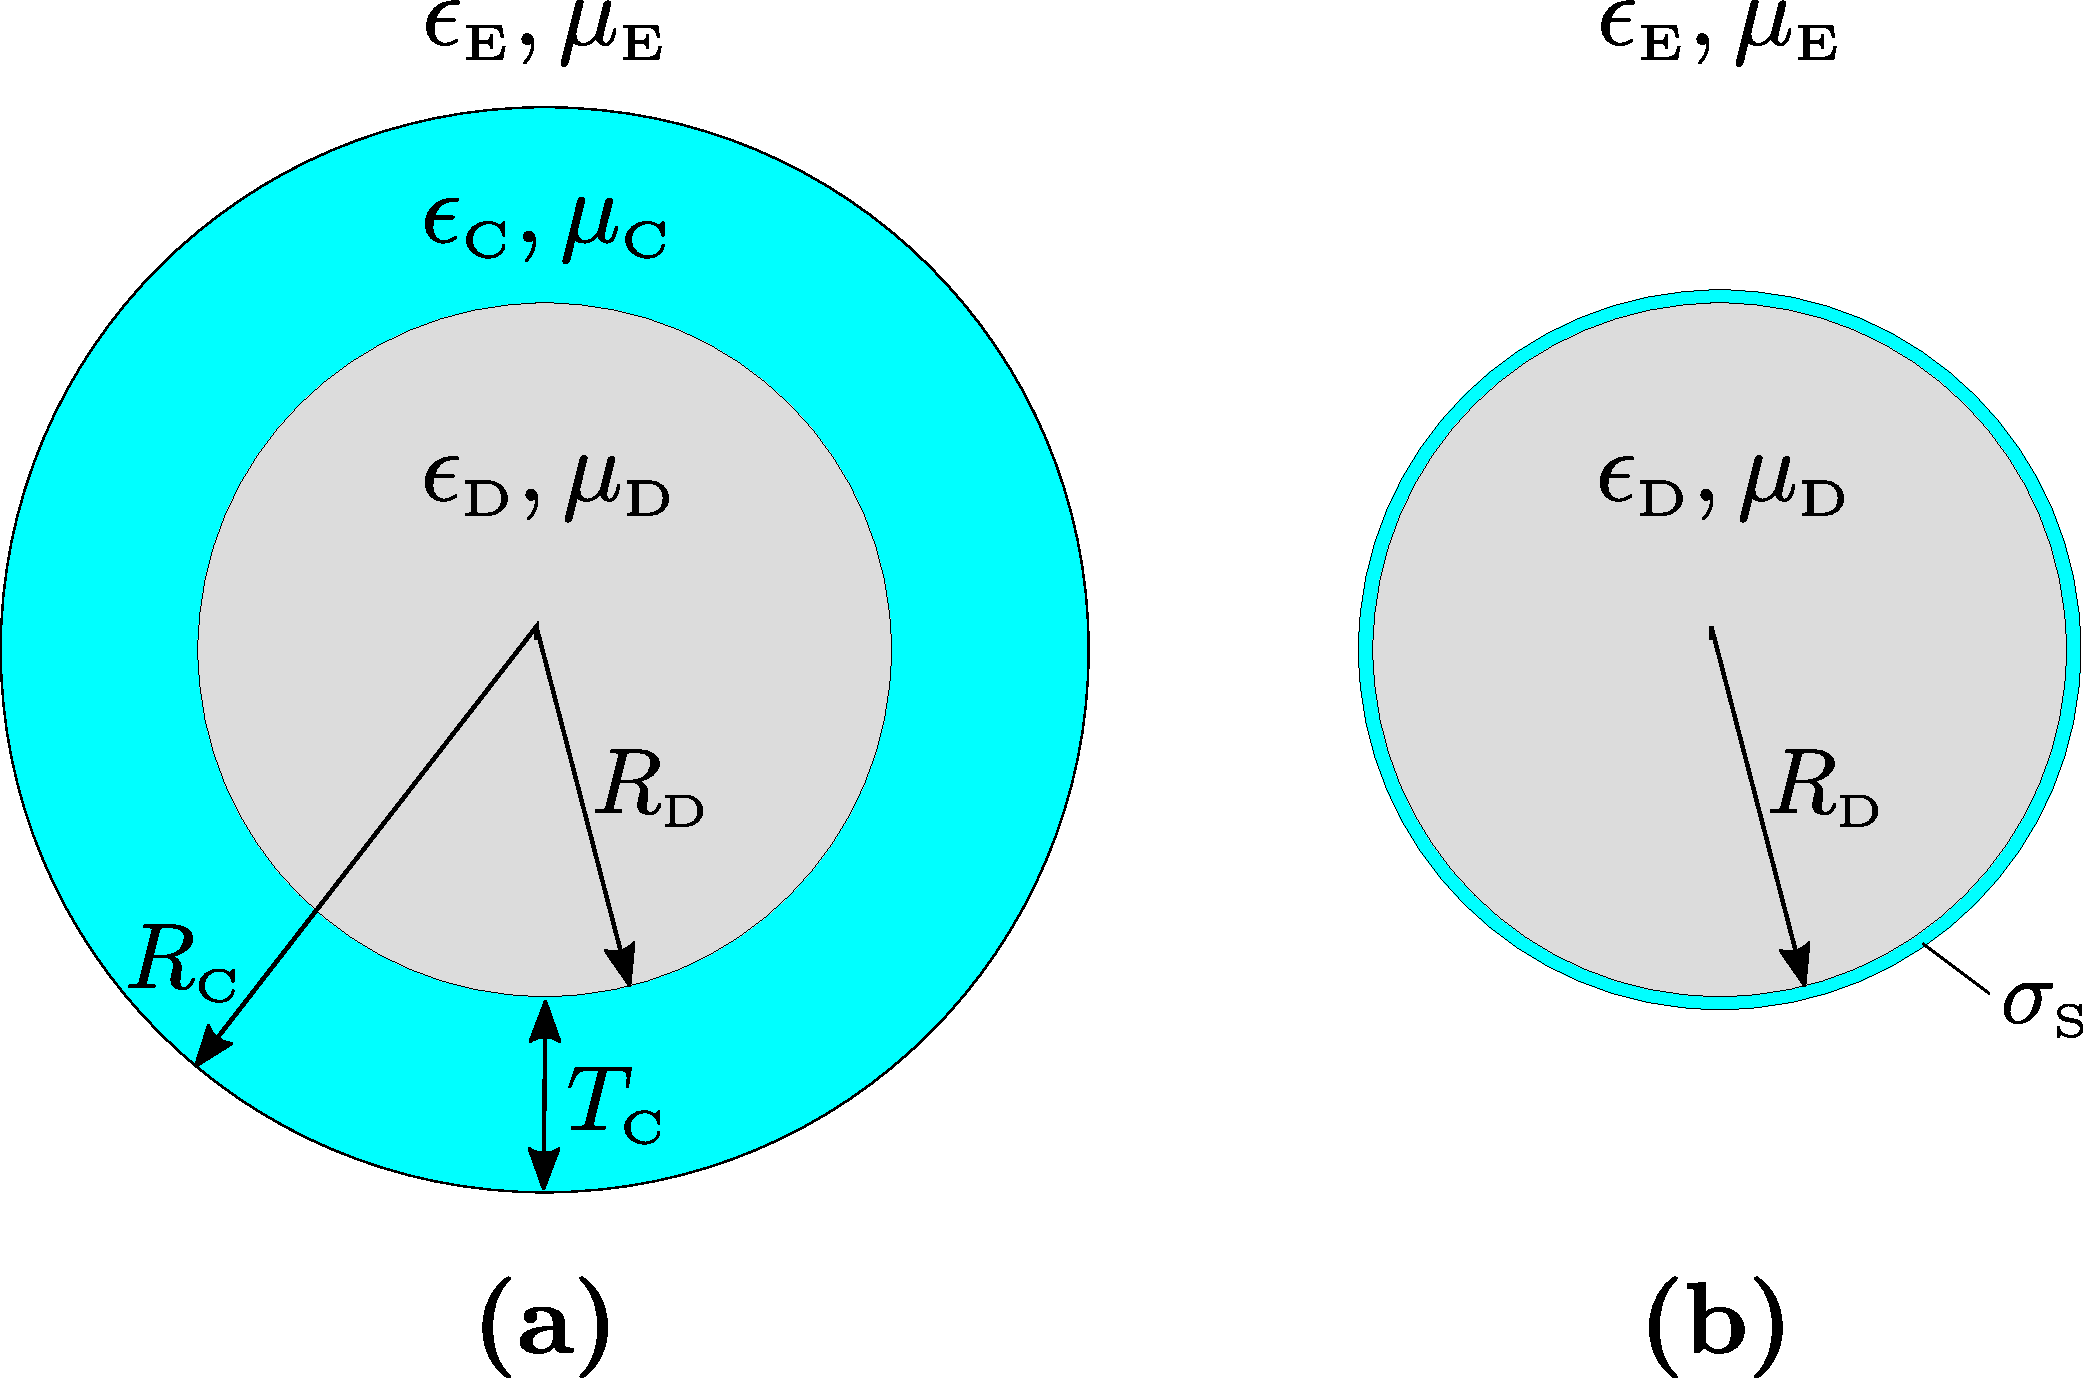
\includegraphics{CoatedSphere.pdf}}
\caption{Dielectric sphere covered by finite-thickness coating layer.
\textbf{(a)} Full geometry.
\textbf{(b)} IBC-layer approximation.
}
\label{CoatedSphereFigure}
\end{figure}
%####################################################################%
%####################################################################%
%####################################################################%
I next consider a spherical version of the geometry of Figure
\ref{TwoFilmFigure}: a dielectric sphere (permittivity
$\epsilon\subt{D}$, radius $R\subt{D}$) coated by a
conducting layer (permittivity $\epsilon\subt{C}$, thickness
$T\subt{C}$) illuminated by a linear combination of regular
spherical waves:\footnote{My conventions for vector spherical
waves are detailed in the companion memo,
``Electromagnetism in the Spherical-Wave Basis''
(\url{http://homerreid.github.io/scuff-em-documentation/tex/scuffSpherical.pdf}).}
%====================================================================%
$$ \vb E\sups{inc}(\vb x)=
   \sum_{\alpha}
     \Big\{ P_\alpha\vb M\sups{reg}_\alpha(\vb x)
            Q_\alpha\vb N\sups{reg}_\alpha(\vb x)
     \Big\}
$$
%====================================================================%

\subsection{Exact solution}
\label{SphereExactSolution}

Fields outside:
%====================================================================%
\begin{subequations}
\begin{align}
 \vb E(\vb x) &= \vb E\sups{inc}(\vb x) 
+ \sum_{\alpha}
     \Big\{ A_\alpha\vb M\sups{out}_\alpha(\vb x)
           +B_\alpha\vb N\sups{out}_\alpha(\vb x)
     \Big\}
\\
\vb H\sups{scat}(\vb x) &= \vb H\sups{inc}(\vb x)
+ \frac{1}{Z_0}
     \sum_{\alpha}
     \Big\{ B_\alpha\vb M\sups{out}_\alpha(\vb x)
           -A_\alpha\vb N\sups{out}_\alpha(\vb x)
     \Big\}
\\
\end{align}
\label{SphereFieldsOutside}
\end{subequations}
%====================================================================%
Fields in conducting layer:
%====================================================================%
\begin{align}
\vb E &= 
   \sum_{\alpha}
     \Big\{ C_\alpha\vb M\sups{out}_\alpha(\vb x)
           +D_\alpha\vb N\sups{out}_\alpha(\vb x)
           +E_\alpha\vb M\sups{reg}_\alpha(\vb x)
           +F_\alpha\vb N\sups{reg}_\alpha(\vb x)
     \Big\}
\\
\vb H &= 
 \frac{1}{Z_0Z\subt{C}}
   \sum_{\alpha}
     \Big\{ D_\alpha\vb M\sups{out}_\alpha(\vb x)
           -C_\alpha\vb N\sups{out}_\alpha(\vb x)
           +F_\alpha\vb M\sups{reg}_\alpha(\vb x)
           -E_\alpha\vb N\sups{reg}_\alpha(\vb x)
     \Big\}
\end{align}
%====================================================================%
Fields inside dielectric sphere:
%====================================================================%
\begin{subequations}
\begin{align}
\vb E &= 
   \sum_{\alpha}
     \Big\{ G_\alpha\vb M\sups{reg}_\alpha(\vb x)
           +H_\alpha\vb N\sups{reg}_\alpha(\vb x)
     \Big\}
\\
\vb H &= 
 \frac{1}{Z_0Z\subt{D}}
   \sum_{\alpha}
     \Big\{ H_\alpha\vb M\sups{reg}_\alpha(\vb x)
           -G_\alpha\vb N\sups{reg}_\alpha(\vb x)
     \Big\}
\end{align}
\label{SphereFieldsInside}
\end{subequations}
%%%%%%%%%%%%%%%%%%%%%%%%%%%%%%%%%%%%%%%%%%%%%%%%%%%%%%%%%%%%%%%%%%%%%%

Match tangential fields:
%%%%%%%%%%%%%%%%%%%%%%%%%%%%%%%%%%%%%%%%%%%%%%%%%%%%%%%%%%%%%%%%%%%%%%
$$\left(\begin{array}{cccc}
    R\sups{out}(R\subt{C})
 & -R\sups{out}(R\subt{C})
 & -R\sups{reg}(R\subt{C})
 & 0
\\
    \RBar\sups{out}(R\subt{C})
 & -\frac{1}{Z\subt{C}}\RBar\sups{out}(R\subt{C})
 & -\frac{1}{Z\subt{C}}\RBar\sups{reg}(R\subt{C})
 & 0
\\
    0   
 &  R\sups{out}(R\subt{D})
 &  R\sups{reg}(R\subt{D})
 & -R\sups{reg}(R\subt{D})
\\
    0   
 & \frac{1}{Z\subt{C}}  \RBar\sups{out}(R\subt{D})
 & \frac{1}{Z\subt{C}}  \RBar\sups{reg}(R\subt{D})
 & -\frac{1}{Z\subt{D}} \RBar\sups{reg}(R\subt{D})
  \end{array}\right)
  \left(\begin{array}{c}
  A \\ C \\ E \\ G
  \end{array}\right)
=-P
  \left(\begin{array}{c}
  R\sups{reg}(R\subt{C}) \\ \RBar\sups{reg}(R\subt{C}) \\ 0 \\ 0
  \end{array}\right)
$$
%%%%%%%%%%%%%%%%%%%%%%%%%%%%%%%%%%%%%%%%%%%%%%%%%%%%%%%%%%%%%%%%%%%%%%  
The equation for the vector $\left(\begin{array}{c}B\\D\\F\\H\end{array}\right)$
is similar with $R\leftrightarrow \RBar$ everywhere.

%%%%%%%%%%%%%%%%%%%%%%%%%%%%%%%%%%%%%%%%%%%%%%%%%%%%%%%%%%%%%%%%%%%%%%
%%%%%%%%%%%%%%%%%%%%%%%%%%%%%%%%%%%%%%%%%%%%%%%%%%%%%%%%%%%%%%%%%%%%%%
%%%%%%%%%%%%%%%%%%%%%%%%%%%%%%%%%%%%%%%%%%%%%%%%%%%%%%%%%%%%%%%%%%%%%%
\subsection{IBC solution}
\label{SphereIBCSolution}

In the IBC version of the problem we have only the fields
(\ref{SphereFieldsOutside}) and (\ref{SphereFieldsInside}).
The IBC condition reads
%====================================================================%
\begin{align*}
 \vb H \big( R\subt{D}^+ \big)
-\vb H \big( R\subt{D}^- \big)
&=-\sigma\subt{S}\vbhat{r}\times E\big(R\subt{D}^-\big)
\intertext{or (using an obvious shorthand)}
Q\vb M\sups{reg} - P\vb N\sups{reg}
+B\vb M\sups{out} - A\vb N\sups{out}
-\frac{1}{Z\supt{D}}H\vb M\sups{reg}
+\frac{1}{Z\supt{D}}G\vb N\sups{reg}
&=-Z_0\sigma\subt{S}\left( G\vbhat{r}\times \vb M\sups{reg} + H\vbhat{r}\times \vb N\sups{reg}\right)
\end{align*}
Noting that 
%====================================================================%
$$ \vbhat{r}\times \vb M\sups{reg} = R\sups{reg} \vb{Z}, \qquad
   \vbhat{r}\times \vb N\sups{reg} = -i\overline{R}\sups{reg} \vb{X}
$$
%====================================================================%
and working through the algebra yields
%====================================================================%
$$
 \left(\begin{array}{cc}
   R\sups{out}(a)
& -R\sups{reg}(na)
\\
   \RBar\sups{out}(a)
& -\frac{1}{Z\subt{D}}\RBar\sups{reg}(na)
  +iZ_0 \sigma\subt{S}R\sups{reg}(na)
 \end{array}\right)
 \left(\begin{array}{c}
 A \\ G 
 \end{array}\right)
=-P
 \left(\begin{array}{c}
  R\sups{reg}(a)
\\
  \RBar\sups{reg}(a)
 \end{array}\right)
$$

$$
 \left(\begin{array}{cc}
  \RBar\sups{out}(a) & -\RBar\sups{reg}(na)
\\ 
   R\sups{out}(a)
& -\frac{1}{Z\subt{D}}R\sups{reg}(na) - iZ_0\sigma\subt{S} \RBar\sups{reg}(na)
 \end{array}\right)
=
   -Q
  \left(\begin{array}{c} \RBar\sups{reg}(a) \\ R\sups{reg}(a)
  \end{array}\right)
$$

%####################################################################%
%####################################################################%
%####################################################################%
\newpage
\section{Implementing conductive dielectric interfaces in {\sc scuff-em}}

The usual $\vb H$-field condition imposed at dielectric boundary surfaces
is\footnote{I am here assuming that the sources of incident field
lie only in the ``outer'' medium.}
%====================================================================%
\begin{align*}
 \vb H_\parallel\sups{out} - \vb H_\parallel\sups{in}
&=0
\intertext{or}
 \vb H_\parallel\sups{scat,out} - \vb H_\parallel\sups{scat,in}
&=-\vb H_\parallel\sups{inc}
\end{align*}
%====================================================================%
If there is a layer of surface conductivity $\sigma\subt{S}$ at the 
interface, the condition is modified to read
%====================================================================%
\begin{align*}
 \vb H_\parallel\sups{out} - \vb H_\parallel\sups{in}
&=-\sigma\subt{S}\vbhat n\times \vb E\sups{in}
\intertext{or}
 \vb H_\parallel\sups{scat,out} - \vb H_\parallel\sups{scat,in}
+\sigma\subt{S}\vbhat n\times \vb E\sups{scat,in}
&=-\vb H_\parallel\sups{inc}
\\
\end{align*}

\end{document}
